\chapter{Unsupervised Learning}

\section{Introduzione}
Nel unsupervised learning non si hanno label per guidare il learning algorithm, pertanto il meccanismo di learning sar\`a molto diverso.
Si osservano i dati da una distribuzione sconosciuta $p_{data}\in\Delta(X)$.
In quanto non si hanno osservazioni riguardo i target si deve introdurre un modello di conoscenza a priori o dare supervisione implicita attraverso il design della funzione obiettivo.

\subsection{Task tipiche}
Le task tipiche dell'unsupervised learning sono:
\begin{itemize}
	\item Dimensionality reduction: incorporare i dati in uno spazio a meno dimensioni.
	\item Clustering: dividere i dati in gruppi con propriet\`a simili.
	\item Density estimation: imparare una distribuzione di probabilit\`a che fitta meglio il training data.
\end{itemize}

\section{Dimensionality reduction}
\subsection{Motivazioni}
Vogliamo comprimere i dati in ingresso riducendone la quantit\`a di features che andiamo a prendere in considerazione, preservando il maggior numero di informazioni possibili. Questo permette di spendere meno tempo nelle fase successive del learning e meno consumo di spazio.
\subsection{Task}
Si deve trovare una funzione $f\in Y^X$ che mappa ogni input a grandi dimensioni $x\in X$ a dimensioni minori incorporando $f(x)\in Y$, dove $dim(Y)\ll dim(X)$.
Questa task permette di preservare le informazioni riducendo la dimensione di ogni dato in input.
Questo approccio permette di visualizzare i dati, semplificare la loro computazione.
Riduce il problema del \emph{curse of dimensionality}.
\subsection{Principal component anlaysis}
In questo meccanismo di dimensionality reduction la conoscenza implicita messa nell'algoritmo \`e che la varianza \`e un indicatore di ricchezza di informazioni dati da una dimensione.
PCA trova una trasformazione ottimale nel sistema di coordinate tale che perdere delle dimensioni nelle nuove coordinante porta la pi\`u piccola riduzione nella varianza dei dati.
PCA in particolare  perde l'asse con la varianza minore perdendo meno informazioni possibile.

\begin{figure}
	\centering
	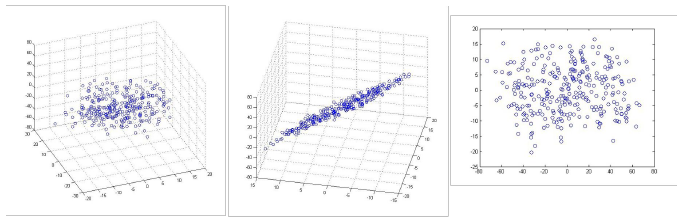
\includegraphics[width=0.6\linewidth]{imgs/chapter12/img0}
	\caption{Idea della dimensionality reduction. Passiamo da 3D a 2D}
	\label{fig:chapter12-00}
\end{figure}

\subsubsection{Varianza lungo una dimensione $\mathbf{w}$}
Per calcolare la varianza lungo una data unit\`a di direzione scegliamo $w$ tale che $w^Tw=1$.
Sia $x_i$ un data point, si necessita di un punto nello spazio $c$ da cui si applica la direzione $w$ per calcolare la varianza di tutti i data points \ref{fig:chapter12-01}:
$$t_i = (x_i-c)^Tw$$


\begin{figure}
	\centering
	\begin{minipage}{.5\textwidth}
		\centering
		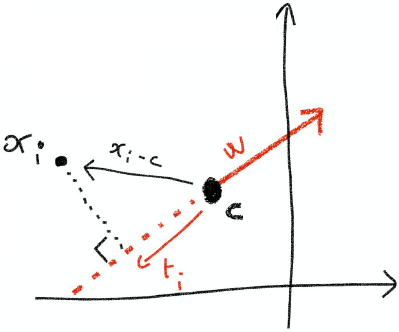
\includegraphics[width=0.6\linewidth]{imgs/chapter12/img1}
		\caption{Varianza lungo una dimensione $\mathbf{w}$}
		\label{fig:chapter12-01}
	\end{minipage}%
	\begin{minipage}{.5\textwidth}
		\centering
		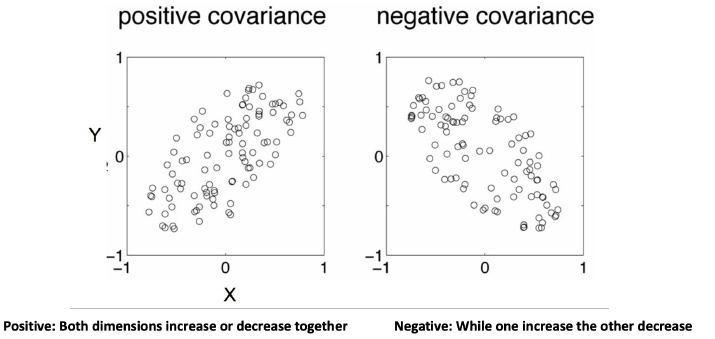
\includegraphics[width=1\linewidth]{imgs/chapter12/img2}
		\caption{Covarianza}
		\label{fig:chapter12-02}
	\end{minipage}
\end{figure}

La proiezione di $x_i$ su $w$.
Il valore atteso $\mathbb{E}[t]$:
\begin{align*}
	\mathbb{E}[t] &= \frac{1}{n}\sum\limits_{i=1}^nt_i = \frac{1}{n}\sum\limits_{i=1}^n(x_i-c)^Tw=\\
	&\bar{x}^Tw-c^Tw
\end{align*}
Ora la varianza sulla dimensione definita da $w$ \`e:
\begin{align*}
	Var[t] &= \frac{1}{n}\sum\limits_{i = 1}^n(t_i -\mathbb{E}[t])^2 = \frac{1}{n}\sum\limits_{i=1}^n[(x_i-\bar{x})^Tw]^2=\\
	&=\frac{1}{n}\sum\limits_{i=1}^n(\bar{x}_i^Tw)^2 = w^T\bigl[\frac{1}{n}\bar{X}\bar{X}^T\bigr]w=\\
	&=w^TCw
\end{align*}
Dove $C$ \`e la matrice della covarianza e $X = [\bar{x}_1,\dots,\bar{x}_n]$.
Si nota come la computazione della varianza non dipende dal punto $c$ in quanto \`e implicitamente calcolata da un punto di vista centrato. La varianza misura la dispersione (spread) dei dati di una determinata variabile intorno alla sua media in una dimensione. La covarianza misura la deviazione dalla media tra due variabili. In altre parole, la covarianza misura la relazione tra due dimensioni. Il segno della covarianza \`e importante: un segno positivo indica una relazione diretta tra le dimensioni confrontate, quindi le due variabili incrementano/decrementano contemporaneamente, un segno negativo indica una relazione indiretta, quindi quando una incrementa l'altra decrementa e viceversa, una correlazione pari a zero indica che non c'\`e relazione tra le dimensioni  \ref{fig:chapter12-02}. Confrontano ogni dimensione con ogni altra andiamo a creare la matrice della covarianza che \`e simmetrica.

\subsubsection{Riassunto eigenvalues e eigenvectors}

Osserva le figure \ref{fig:chapter12-03} e \ref{fig:chapter12-04}.

\begin{figure}
	\centering
	\begin{minipage}{.6\textwidth}
		\centering
		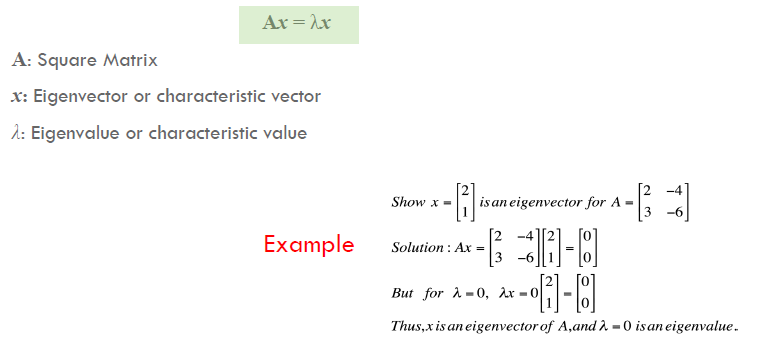
\includegraphics[width=1\linewidth]{imgs/chapter12/img3}
		\caption{}
		\label{fig:chapter12-03}
	\end{minipage}%
	\begin{minipage}{.4\textwidth}
		\centering
		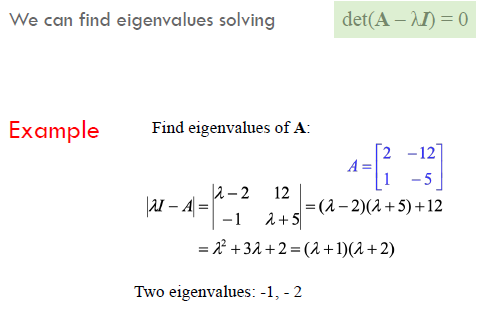
\includegraphics[width=1\linewidth]{imgs/chapter12/img4}
		\caption{}
		\label{fig:chapter12-04}
	\end{minipage}
\end{figure}

\subsubsection{Eigenvalue decomposition}
Sia $A\in R^{m\times m}$ quadrata e simmetrica.
Allora esiste $U=[u_1,\dots,u_n]\in R^{m\times m}$ e $\lambda=(\lambda_1,\dots,\lambda_m)^T\in R^m$ tali che:
$$A = U\Lambda U^T=\sum\limits_{j=1}^m\lambda_ju_ju_j^T$$
E $U^TU=UU^T=I$ e $U$ \`e ortonormale.
Ogni colonna di $U$ ha lunghezza di unit\`a e ogni paio di colonne diverse sono ortogonali tra di loro.
La matrice $\Lambda$ \`e creata con zero da tutte le parti e $\lambda$ sulla diagonale principale.
$u_j$ \`e un eigenvector e $\lambda_j$ \`e la eigenvalue corrispondente.
Si assume un ordinamento discendente: $\lambda_1\ge \lambda_m$.

\subsubsection{First principal component}
Il first principal component \`e la direzione dove la maggior parte della varianza \`e conservata.
Si deve risolvere il problema di massimizzazione della varianza:
$$w_1\in arg\max\{w^TCw:w^Tw=1\}$$
Si devono fare costraints su $w_1$ altrimenti crescerebbero all'infinito.
La varianza di PCA \`e il valore del pi\`u grande eigenvalue della matrice $C$ di covarianza, la prima componente principale \`e il corrispondente vettore $w_1$.
Il maggiore eigenvalue di $C$ \`e la varianza lungo il first principal component e il first principal component $w_1$ \`e il corrispondente eigenvector.

\paragraph{Dimostrazione}
Dalla decomposizione di eigenvalue $C=\sum\limits_j\lambda_ju_ju_j^T$ si assumono le eigenvalue ordinate in ordine discendente.
Allora $W_1^TCw_1 = \sum\limits_j\lambda_j(w_1^Tu_j)^2\le\lambda_1$ in quanto:
$$\sum\limits_j(w_1^Tu_j)^2 = w_1^T\sum\limits_ju_ju_j^Tw_1=w_1^TUU^Tw_1=w_1^Tw_1=1$$
Segue che $\lambda_1\ge w_1^TCw_1 >u_1^TCu_1=\lambda_1$, da cui $w_1^TCw_1=u_1^TCu_1$.
Pertanto $u_1$, l'eigenvector corrispondente al eigenvalue maggiore $\lambda_1$ di $C$ \`e il first principal componente e $\lambda_1$ la varianza lungo di esso.

\subsubsection{Second principal component}
Il second principal component deve essere ortogonale al primo:
$$w_2\in arg\{w^TCw:w^Tw=1,w\perp w_1\}$$
Il secondo eigenvalue maggiore di $C$ \`e la varianza lungo il second principal component e $w_2$ \`e il corrispondente eigenvector.

\paragraph{Dimostrazione}

Dalla decomposizione di eigenvalue $C=\sum\limits_j\lambda_ju_ju_j^T$ si assumono le eigenvalue ordinate in ordine discendente.
Allora
$$W_2^TCw_2 = \sum\limits_{j=1}^m\lambda_j(w_2^Tu_j)^2=\lambda_1w_2^Tu_1+\sum\limits_{j=2}^m\lambda_j(w_2^Tu_j)^2\le\lambda_2$$
In quanto:
$$\sum\limits_j(w_2^Tu_j)^2 = w_2^T\sum\limits_ju_ju_j^Tw_2=w_2^TUU^Tw_2=w_2^Tw_2=1$$
Segue che $\lambda_2\ge w_2^TCw_2 >u_2^TCu_2=\lambda_2$, da cui $w_2^TCw_2=u_2^TCu_2$.
Pertanto $u_2$, l'eigenvector corrispondente al secondo eigenvalue maggiore $\lambda_2$ di $C$ \`e il second principal componente e $\lambda_2$ la varianza lungo di esso.

\subsubsection{Iesimo principal component}
Allo stesso modo:
$$w_i\in arg\{w^TCw:w^Tw=1,w\perp w_j 1\le j < i\}$$
L'i-esimo eigenvalue maggiore di $C$ \`e la varianza lungo l'iesimo principal component.
L'iesimo principal component \`e $w_i$ \`e il corrispondente eigenvector.
La dimostrazione \`e analoga a quella del second principal component.

\subsubsection{PCA utilizzando eigenvalue decomposition}
\begin{itemize}
	\item Siano i data points $X=[x_1,\dots,x_n]$.
	\item Si centri $\bar{X} = X-\frac{1}{n}X1_n1_n^T$.
	\item Si computi la matrice di covarianza $C=\frac{1}{n}\bar{X}\bar{X}^T$.
	\item Eigenvalue decomposition: $U,\lambda = eig(C)$.
	\item Principal components: $W=U=[u_1,\dots,u_m]$, varianze $\lambda = (\lambda_1,\dots,\lambda_m)$.
\end{itemize}

\subsubsection{PCA utilizzando singular value decomposition (SVD)}
Sia $A\in\mathbb{R}^{m\times n}$.
Allora esiste $U\in\mathbb{R}^{m\times k}$, $s\in\mathbb{R}^k$ con $s_1\ge\cdots\ge s_K >0$ e $V\in \mathbb{R}^{n\times k}$ tali che:
$$A = USV^T\qquad\qquad\land\qquad\qquad U^TU=V^TV=I$$
Si computa pertanto la SVD di $\bar{X}:U,s,V=SVD(\bar{X})$.
Le componenti principali $U=[u_1,\dots,u_k]$ e le varianze $\bigl(\frac{s_1^2}{n},\dots,\frac{s_k^2}{n}\bigr)$
La matrice $U$ \`e la matrice con gli eigenvectors.
Le eigenvalue possono essere calcolate in quanto: $\bar{x} = USV^T$ e $c = \frac{1}{n}\bar{x}\bar{x}^T = \frac{1}{n}USV^TVSU^T=U\frac{s^2}{n}u^T$

\subsubsection{Dimensionality reduction}
Sia $\hat{W} = [w_1,\dots,w_k]$ le prime $k$ componenti principali derivate dai data points $\bar{X} = [\bar{x}_1,\dots,\bar{x}_n]$.
Si cambia a un sistema di coordinate ridotto con le $k$ componenti principali con $\hat{W}$ come assi:
$$T = \hat{W}^T\bar{X}\in\mathbb{R}^{k\times n}$$
Dove $T$ \`e il principal component scores.
Si pu\`o usare la eigenvalue decomposition o SVD per computare la decomposizione completa.
Con la PCA si ottengono gli eigenvectors o componenti, si possono ordinare e usarli per comporre la matrice $\hat{W}$.
Una volta fatto quello si usa per calcolare $T$ che \`e il dataset dimensionalmente ridotto.

\subsubsection{Interpretazioni alternative}
Si pu\`o considerare la first principal component come la linea nello spazio con la minore distanza quadrata dai data points.
La stessa interpretazione pu\`o essere data alle altre componenti principali.

\subsubsection{Scalare delle variabili}
PCA \`e sensibile alla scala delle features, pertanto \`e raccomandato scalarle secondo la standard deviation.

\subsubsection{Esempio}

Per un esempio osserva le figure \ref{fig:chapter12-05}, \ref{fig:chapter12-06}, \ref{fig:chapter12-07}, \ref{fig:chapter12-08} e \ref{fig:chapter12-09}.


\begin{figure}
	\centering
	\begin{minipage}{.5\textwidth}
		\centering
		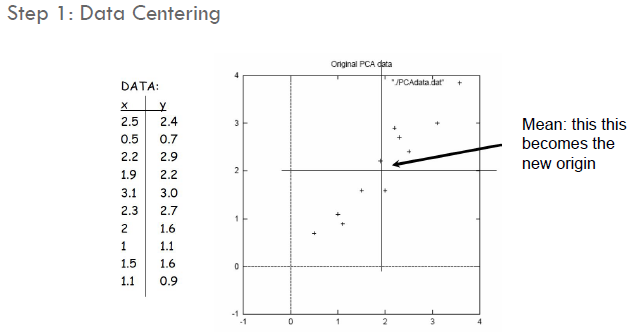
\includegraphics[width=1\linewidth]{imgs/chapter12/img5}
		\caption{}
		\label{fig:chapter12-05}
	\end{minipage}%
	\begin{minipage}{.5\textwidth}
		\centering
		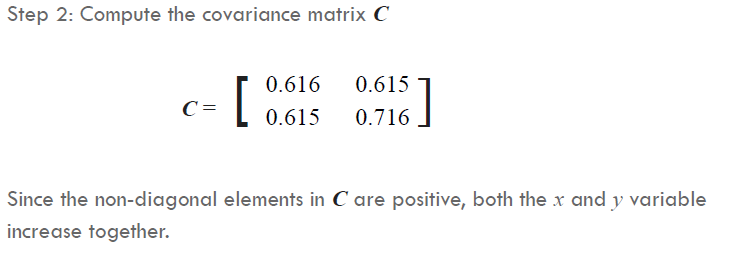
\includegraphics[width=1\linewidth]{imgs/chapter12/img6}
		\caption{}
		\label{fig:chapter12-06}
	\end{minipage}
\end{figure}

\begin{figure}
	\centering
	\begin{minipage}{.5\textwidth}
		\centering
		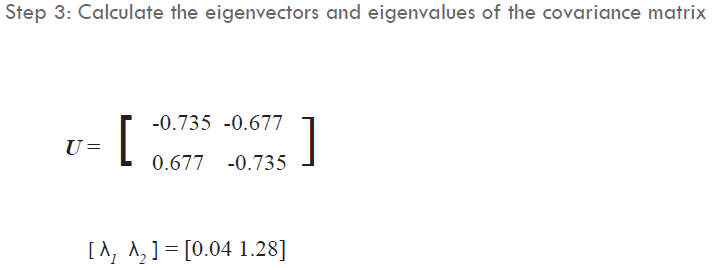
\includegraphics[width=1\linewidth]{imgs/chapter12/img7}
		\caption{}
		\label{fig:chapter12-07}
	\end{minipage}%
	\begin{minipage}{.5\textwidth}
		\centering
		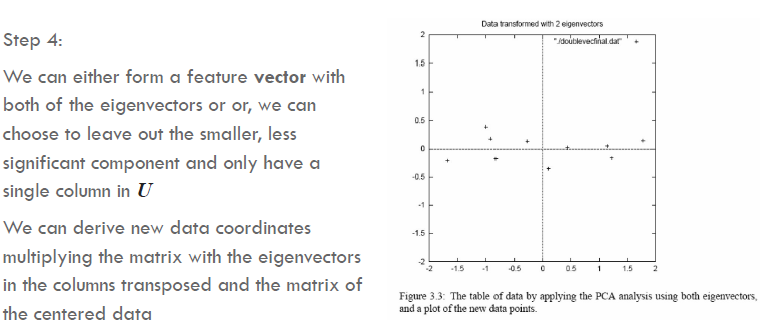
\includegraphics[width=1\linewidth]{imgs/chapter12/img8}
		\caption{}
		\label{fig:chapter12-08}
	\end{minipage}
\end{figure}

\begin{figure}
	\centering
	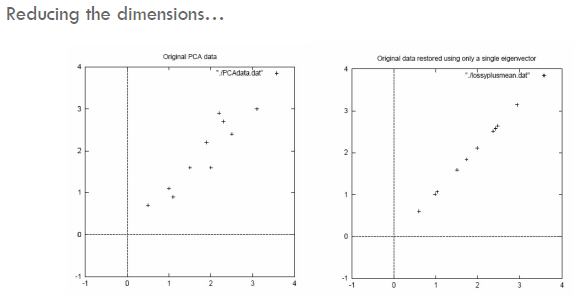
\includegraphics[width=0.6\linewidth]{imgs/chapter12/img9}
	\caption{}
	\label{fig:chapter12-09}
\end{figure}

\subsubsection{Componenti principali da considerare}
Il numero di componenti per la dimensionality reduction dipende dall'obiettivo e dall'applicazione.
Non ci sono modi per validarla a meno di volerla usare in un contesto di un modello con supervision, ma si pu\`o calcolare la proporzione cumulativa di varianza spiegata che per i primi principal component \`e:
$$\frac{\sum\limits_{j = 1}^k\lambda_j}{\sum\limits_{j = 1}^m C_{jj}}$$
A parole: stiamo riducendo da m a k dimensioni, se il risultato \`e alto, per esempio 0.99 significa che riducendo da m a k dimensioni siamo comunque in grado di spiegare bene di dati, un numero pi\`u basso indica che stiamo perdendo troppe informazioni.
Per la eigenvalue decomposition \`e:
$$\frac{\sum\limits_{j = 1}^ks^2_j}{\sum\limits_{ij} \bar{X}^2C_{ji}}$$
Queste formule permettono di stimare la quantit\`a di informazione persa calcolando la percentuale di varianza che si \`e mantenuta riducendo la dimensionalit\`a dei dati.

\subsubsection{Kernel PCA}
La PCA riduce la dimensionalit\`a attraverso una trasformazione lineare.
Pertanto utilizzando il kernel trick si pu\`o applicare una PCA in uno spazio a pi\`u dimensioni ottenendo una trasformazione non lineare nello spazio originale \ref{fig:chapter12-10}.
\begin{figure}
	\centering
	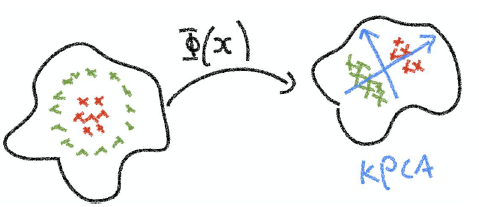
\includegraphics[width=0.6\linewidth]{imgs/chapter12/img10}
	\caption{Kernel PCA. La funzione sar\`a calcolata implicitamente utilizzando il kernel}
	\label{fig:chapter12-10}
\end{figure}
\section{Altre tecniche di dimensionality reduction}
\begin{itemize}
	\item PCA (Principal Component Analysis): Trova la proiezione che massimizza la varianza
	\item Multidimensional Scaling: Trovare la proiezione che meglio preserva le distanze interpunto distanze tra i punti 
	\item LDA (Linear Discriminant Analysis): Massimizzazione degli assi delle componenti per separazione delle classi
\end{itemize}

\section{Applicazioni del PCA}
Come detto in precedenza la PCA pu\`o essere utilizzata per risolvere il problema del riconoscimento facciale. Tratteremo i pixel delle immagini come vettori e andremo in fine a cercare l'immagine pi\`u simile con una ricerca nearest-neighbor. Le immagini di per se sono estremamente di alte dimensioni, con immagini di 100x100 pixel si raggiungono dimensioni nelle decine di centinaia di valori per ogni immagine, ma solo pochi vettori di 10000 dimensioni sono immagini valide. Possiamo trovare il migliore sottospazio dei vettori di 10000 dimensioni dove i vettori sono immagini di facce.

\section{Clustering}
\subsection{Task}
Si deve trovare una funzione $f\in N^X$ che assegna ogni input $x\in X$ a un indice di cluster $f(x)\in N$.
Tutti i punti mappati allo stesso indice formano un cluster.
Ci sono diversi tipi di cluster: partizionali, gerarchici e overlapped.
Permette di trovare gruppi di dati con delle propriet\`a interne, comprimere i dati riducendo il numero di data points invece di ridurre la dimensionalit\`a delle features.	

\subsection{K-means clustering}
Il K-means clustering richiede di sapere prima il numero $k$ di gruppi in cui si vogliono dividere i dati.
Siano i data points $X=[x_1,\dots,x_n]\in\mathbb{R}^{d\times n}$.
Fissato un numero di cluster $k$, si vuole trovare una partizione di data points in $k$ insiemi $\mathcal{L}_1,\dots,\mathcal{L}_k$ che minimizza la variazione $V(\mathcal{L}_j)$ in ogni set $\mathcal{L}_j$
$$\min\limits_{\mathcal{L}_1,\dots,\mathcal{L}_K}\sum\limits_{j = 1}^kV(\mathcal{L}_j)$$
La variazione \`e tipicamente data da $V(\mathcal{L}_j) = \sum\limits_{i\in\mathcal{L}_j}||x_i-\mu_j||^2$, dove $\mu_j = \frac{1}{|\mathcal{L}_j|}\sum\limits_{i\in\mathcal{L}_j}x_i$, il centroide di $\mathcal{L}_j$.
Si deve definire una funzione obiettivo che minimizza la somma di variazioni in ogni set creato.
L'algoritmo di ottimizzazione \`e semplice, inizializza con centroidi casuali e poi mentre i cluster cambiano assegna ogni datapoint al centroide pi\`u vicino formando nuovi cluster e computando nuovi centroidi \ref{fig:chapter12-11}.
\begin{figure}
	\centering
	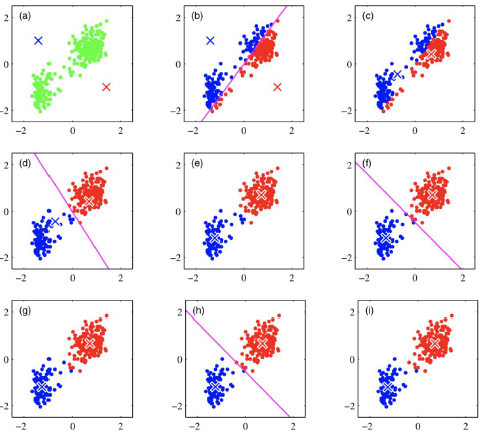
\includegraphics[width=0.6\linewidth]{imgs/chapter12/img11}
	\caption{Esempio. Partiamo da due punti casuali e poi raffiniamo le scelte}
	\label{fig:chapter12-11}
\end{figure}

Questo algoritmo ha una convergenza garantita in quanto migliora strettamente la assignment di cluster e siccome sono finiti a un certo punto converge per forza.
Non \`e comunque garantito trovi il minimo in quanto \`e un problema NP-hard anche sul piano, troveremo un minimo locale.
\`E sensibile alla scala delle features: in alcuni casi avremo bisogno di una funzione di normalizzazione delle features.

\subsubsection{Distanza}
La distanza euclidea:
$$d(x,y) = \sqrt{\sum\limits_{i=1}^n(x_i-y_i)^2}$$
Non \`e sempre una buona scelta: per esempio, nel fare clustering di documenti si sceglie una feature per ogni parola e il valore \`e il numero di volte che tale parola compare.
Si nota come qui due distribuzioni possono avere una grande distanza ma distribuzioni simili.

\paragraph{Cosine similarity}
Per risolvere questo problema si utilizza la cosine similarity:
$$sim(x,y) = \frac{x\cdot y}{|x||y|} = \frac{x}{|x|}\cdot\frac{y}{|y|} = \frac{\sum\limits_{i = 1}^n x_iy_i}{\sqrt{\sum\limits_{i = 1}^n x_i^2}\sqrt{\sum\limits_{i = 1}^ny_i^2}}$$
Questa \`e correlata con l'angolo tra due vettori.
Varia tra $0$ e $1$.
\`E buona per dati di testo e molti altri.
Di facile computazione in quanto si possono considerare solo features con valori non zero in entrambi gli esempi.
La cosine distance:
$$d(x,y) = 1-sim(x,y)$$

\subsubsection{Propriet\`a di K-means}

\paragraph{Convergenza}
L'algoritmo \`e garantito che converga in quanto migliora strettamente l'obiettivo se c'\`e almeno un cambio di cluster e l'insieme delle partizioni \`e finito.
Questo avviene in quanto durante il primo step di assignment ogni altro assignment causerebbe una loss maggiore e durante la computazione del centroide la media di un insieme di valori minimizza l'errore quadratico.

\paragraph{Minimo}
Non \`e garantito che trovi il minimo globale ma uno locale.
Questo avviene in quanto tipicamente la loss function \`e non convessa.

\paragraph{Selezione dei centroidi}
I risultati possono variare enormemente sulla scelta dei centroidi con random seed selection: alcuni possono causare povera convergenza o convergenza a cluster sub-ottimali.
Alcune euristiche comuni sono:
\begin{multicols}{2}
	\begin{itemize}
		\item Punti casuali nello spazio.
		\item Esempi scelti casualmente.
		\item Punti meno simili a ogni centro esistente.
		\item Si provano diversi punti di inizio.
		\item Si inizializza con i risultati di un altro metodo di clustering.
	\end{itemize}
\end{multicols}

\subsection{Problematiche del clustering}
Il clustering presenta diverse problematiche:
\begin{multicols}{2}
	\begin{itemize}
		\item Rappresentazione di un esempio per il cluster.
		\item Simiglianza e distanza tra esempi.
		\item Clustering piatto o gerarchico.
		\item Numero di cluster fisso o data driven.
	\end{itemize}
\end{multicols}

\subsection{Algoritmi di clustering}

\subsubsection{Flat algorithms}
Tipicamente iniziano con un partizionamento causale parziale che viene raffinato iterativamente.
Sono per esempio K means, model based e spectral.

\subsubsection{Hierarchical algorithms}
Si dividono in agglomerativi bottom-up o divisivi top-down.

\subsubsection{Hard clustering}
Nell'hard clustering ogni esempio appartiene esattamente ad un cluster.

\subsubsection{Soft clustering}
Nel soft clustering ogni esempio pu\`o appartenere a pi\`u di un cluster.
\`E pertanto probalistico.

\subsection{EM clustering}
Si nota come il K-means clustering assume sempre dei cluster circolari.
Per questo EM clustering assume che i dati vengano da un'insieme di gaussiane: sono cos\`i ellittici.
Ogni dato viene assegnato a un cluster con una certa probabilit\`a: soft clustering.
\`E molto simile a un alto livello a K-means: itera tra assigning points e ricalcolando i centri dei cluster.
Le differenze principali sono che si assumano cluster ellittici e che sia un algoritmo di soft-clustering.
Pertanto si inizia con dei centri di cluster iniziale, successivamente si assegnano soft points ad ogni cluster calcolando $p(\theta_c|x)$ la probabilit\`a che ognuno di essi appartenga a un cluster \ref{fig:chapter12-12}.
Si ricalcolano i centri del cluster con nuovi parametri $\theta_c$, la massima probabilit\`a dei centri dati il corrente soft clustering.
I centri ottengono una contribuzione pesata dai punti.
\begin{figure}
	\centering
	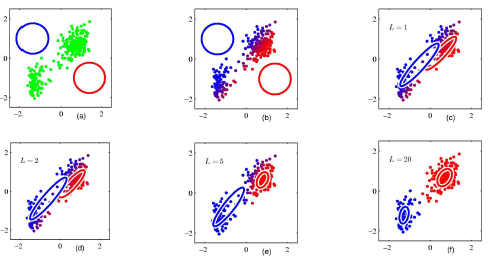
\includegraphics[width=0.8\linewidth]{imgs/chapter12/img12}
	\caption{Esempio}
	\label{fig:chapter12-12}
\end{figure}

\subsubsection{Mixture of Gaussians}
In una dimensione una gaussiana:
$$f(x;\sigma;\mu) = \frac{1}{\sigma\sqrt{2\pi}}e^{-\frac{(x-\mu)^2}{2\sigma^2}}$$
In $m$ dimensioni invece:
$$N[x;\mu;\Sigma] = \frac{1}{(2\pi)^{\frac{d}{2}}\sqrt{det(\Sigma)}}e^{[-\frac{1}{2}(x-\mu)^T\Sigma^{-1}(x-\mu)]}$$
Si impara pertanto la media di ogni cluster o suo centro e la matrice di covarianza, ovvero quanto si disperde, la forma del contorno.

\subsubsection{Soft cluster points}
Si assegna soft ogni punto a ogni cluster calcolando $p(\theta_c|x)$ o la probabilit\`a di ogni punto di appartenere al cluster.
Si utilizza l'equazione della Gaussiana per ogni cluster normalizzata per creare una probabilit\`a.

\subsubsection{Ricalcolo dei centri}
Si calcolano nuovi parametri di cluster $\theta_c$.
Il maximum likelihood cluster center dati il soft clustering corrente.
Questo si fa fittando una gaussiana.

\paragraph{Fit di una gaussiana}
Si fa calcolando la media $\mu$ e la varianza $\sigma$ dei dati.

\subsubsection{Conclusione}
EM clustering sta per expectation maximization.
Per expectation si intende dato il modello corrente, si trova le probabilit\`a aspettate dei data points ad ogni cluster.
La massimizzazione \`e dato l'assignment probabilistico di tutti i punti la stima del nuovo modello $\theta_c$.
Come $k$-means \`e garantito che converga ad un ottimo locale, \`e un algoritmo general purpose per fare training di un modello senza labels.

\subsection{Altri algoritmi di clustering}
K-means e EM-clustering non possono gestire tutte le task di clustering.
In particolare non possono gestire dati non distribuiti secondo una gaussiana, soffrono dello stesso problema dei modelli lineari in quanto non sono in grado di prendere decisioni locali.

\subsubsection{Spectral clustering}
Nello spectral clustering avviene una partizione a grafo: si definisce una matrice di somiglianza e si taglia il grafo.

\subsubsection{Clustering gerarchico}
Il clustering gerarchico produce un insieme di cluster nested organizzati come un albero gerarchico detto dendrogram.
Viene tipicamente utilizzato per i profili genici.

\section{Density estimation}

\subsection{Task}
Si deve trovare una distribuzione di probabilit\`a $f\in \Delta(X)$ che fitta i dati $x\in X$.
Permette di ritornare una stima esplicita della distribuzione di probabilit\`a che genera i dati.
Permette la generazione di nuovi dati dalla stessa distribuzione e l'individuazione di anomalie.

\subsection{Generative model}
I generative model risolvono la task della density estimation.
Sono modelli statistici della distribuzione dei dati sull'input $p_x$ o di una joint distribution sulla coppia di input label $p_{XY}$ dipendente dalla disponibilit\`a dei dati obiettivo.
La loro abilit\`a principale \`e di generare nuovi dati dalle distribuzioni osservate. Immagine di aver allenato un modello fornendo una grande quantit'a di immagini di gatti, ad un certo punto il modello avr'a imparato cosa rende un gatto, un gatto, per esempio la forma, il colore, e dato in input un immagine con solo rumore casuale, generare un gatto simile a quelli visti in precedenza.

\subsection{Modelli discriminativi}
I modelli discriminativi sono modelli statistici della distribuzione di probabilit\`a condizionale $p_{Y|X}$ del target dato l'input.
Tipicamente svolgono una task di classificazione come SVM, decision trees e classificatori KNN. Un esempio \`e un modello in grado di distinguere immagini di cani e gatti e data un'immagine il modello fornisce una confidenza che nella data immagine sia rappresentato un cane o un gatto.
Un modello discriminativo pu\`o essere costruito da uno generativo attraverso la regola di Bayes ma non viceversa:
$$p_{Y|X}(x) = \dfrac{p_{XY}(x,y)}{\sum\limits_{y'}p_{XY}(x,y')p_X(x)}$$

\subsection{Tipi di density estimation}
Per entrambi i modi si trovano due tipi della task:
\begin{itemize}
	\item Supervised: $Z\in X\times Y$.
	\item Unsupervised $Z\in X$.
\end{itemize}

\subsubsection{Explicit density estimation}
Si deve trovare una distribuzione di probabilit\`a $f\in \Delta(Z)$ che fitta i dati $z\in Z$ dove $z$ \`e campionato da una distribuzione di dati sconosciuta $p_{data}\in\Delta(Z)$ \ref{fig:chapter12-18}.

\subsubsection{Implicit density estimation}
Si vuole trovare una funzione $f\in Z^\Omega$ che genera i dati $f(\omega)\in Z$ da un input $\omega$ campionato da una distribuzione predefinita $p_\omega\in\Delta(\Omega)$ in modo che la distribuzione del campione generato fitta la distribuzione sconosciuta $p_{data}\in\Delta(Z)$.
Non si stima la probabilit\`a $\omega$ ma ci si concentra unicamente sul riprodurre i dati con la stessa distribuzione di quella sconosciuta originaria \ref{fig:chapter12-19}.

\begin{figure}
	\centering
	\begin{minipage}{.5\textwidth}
		\centering
		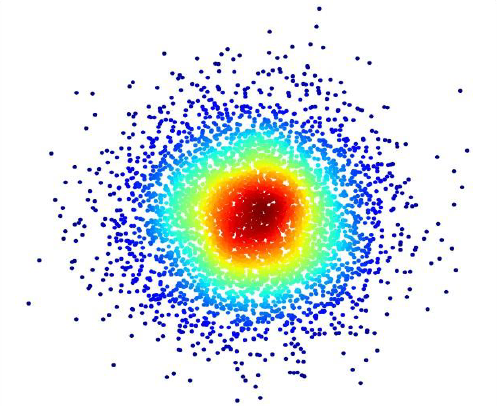
\includegraphics[width=0.7\linewidth]{imgs/chapter12/img18}
		\caption{Explicit density estimation}
		\label{fig:chapter12-18}
	\end{minipage}%
	\begin{minipage}{.5\textwidth}
		\centering
		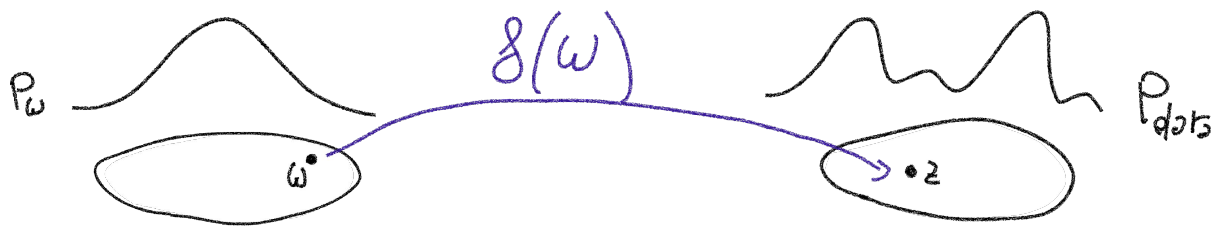
\includegraphics[width=1\linewidth]{imgs/chapter12/img19}
		\caption{Implicit density estimation}
		\label{fig:chapter12-19}
	\end{minipage}
\end{figure}


\subsubsection{Obiettivo per i modelli generativi}
Si deve definire uno spazio di ipotesi $H\subset \Delta(Z)$, consiste di un insieme di modelli che possono rappresentare distribuzioni di probabilit\`a definite esplicitamente o implicitamente.
Si definisce una misura di divergenza $d\in R_+^{\Delta(Z)\times\Delta(Z)}$ tra le distribuzione di probabilit\`a in $\Delta(Z)$ e si usa la divergenza di Kullback-Leibler.
La divergenza \`e $0$ se due distribuzioni hanno un match, altrimenti \`e negativa.
L'algoritmo tenta di trovare $q^*\in H$ che ha un fit migliore sui dati distribuiti secondo $p_{data}$ dove il best fit \`e quello con la divergenza minore.
$$q^*\in arg\min\limits_{q\in\mathcal{H}}d(p_{data},q)$$
Si assumer\`a che la distribuzione dei dati \`e solo su $X$ con unsupervised learning, ma il trasporto a supervised \`e banale.

\subsection{Variational AutoEncoder (VAE)}
Un autoencoder \`e un modo per comprimere dati ad alta dimensione in una rappresentazione a meno dimensioni: dimensionality reduction.
Un encoder mappa i dati di input $x$ a una rappresentazione compressa $\omega$.
La rappresentazione conserva fattori significativi nella variazione dei dati come in PCA.

\subsubsection{Training}
Un encoder viene trainato creando un decoder che mappa la rappresentazione di $\omega$ indietro nel dominio di input portando a una ricostruzione $\hat{x}$.
Pertanto l'encoder autoencoda il proprio input.
L'obiettivo \`e quello di minimizzare la divergenza tra l'input $x$ e la sua ricostruzione $\hat{x}$ che porta all'algoritmo di training verso la minima perdita di informazione durante la fase di encoding.
Dopo il training il decoder non \`e pi\`u necessario in quanto \`e funzionale solo per stimare l'encoder.
L'encoder invece pu\`o essere utile per diverse tasks, per esempio per inizializzare o precomputare le caratteristiche per supervised models.

\subsubsection{Generare dati con il decoder}
Il decoder potrebbe essere usato per generare nuovi dati ma non li generer\`a secondo $p_{data}$ in quanto niente lo obbliga.
Se si genera un input a caso $\omega$ non si \`e sicuri che $\omega$ \`e una combinazione che verrebbe ordinata dalla distribuzione dei dati.
La soluzione a questo problema sarebbe di avere una distribuzione a priori $\Omega$ che ci dice la probabilit\`a di campionare ogni $\omega$ dallo spazio encodato.
Il decoder poi sarebbe capace di tradurre la distribuzione $\Omega$ nella distribuzione di dati in $X$ \ref{fig:chapter12-13}.
\begin{figure}
	\centering
	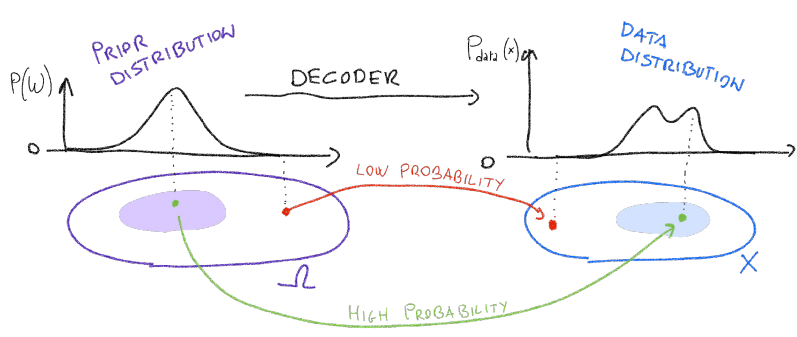
\includegraphics[width=0.6\linewidth]{imgs/chapter12/img13}
	\caption{Cosa vorremmo}
	\label{fig:chapter12-13}
\end{figure}

\paragraph{Training del decoder}
In termini formali il decoder: $q_\theta(x|\omega)$ \`e una distribuzione di probabilit\`a $x$ per ogni valore $\omega$.
La probabilit\`a a priori \`e $p_\omega$
Si pu\`o ottenere un'aspettativa marginalizzata
$$q_\theta(x) = \mathbb{E}_{\omega\sim p_\omega}[q_\theta(x|\omega)]$$
Successivamente si pone come obiettivo modificare il parametro $\theta$ per minimizzare la divergenza tra la distribuzione dei dati e $q_\theta$:
$$\theta^*\in arg\min\limits_{\theta\in\Theta}d(q_\theta,p_{data})$$
Si utilizza KL-divergence.
\`E non negativa e $0$ se $p$ e $q$ sono la stessa distribuzione.
$$d_{KL}(p,q) = \mathbb{E}_{x\sim p}\bigl[\log\frac{p(x)}{q(x)}\bigr]$$

\paragraph{Intrattabilit\`a}
Analizzando la divergenza si vede che il suo calcolo \`e intrattabile a causa del valore atteso:
\begin{align*}
	d_{KL}(p_{data}, q_\theta) &= \mathbb{E}_{x\sim p_{data}}\bigl[\log\frac{p_{data}(x)}{q_\theta(x)}\bigr]=\\
	& = -\mathbb{E}_{x\sim p_{data}}[\log q_\theta(x)] + const=\\
	&= -\mathbb{E}_{x\sim p_{data}}[\log\mathbb{E}_{\omega\sim p_\omega} [q_\theta(x|\omega)]]+const
\end{align*}
Si pu\`o approssimare il valore atteso attraverso stochastic gradient descent.
\begin{align*}
	\frac{d}{d\theta}d_{KL}(p_{data},q_\theta) &= -\frac{d}{d\theta}\mathbb{E}_{x\sim p_{data}}[\log\mathbb{E}_{\omega\sim p_\omega}[q_\theta(x|\omega)]=\\
	& = -\mathbb{E}_{x\sim p_{data}}\bigl[\frac{d}{d\theta}\log\mathbb{E}_{\omega\sim p_\omega}[q_\theta(x|\omega)]\bigr]=\\
	& = - \mathbb{E}_{x\sim p_{data}}\biggl[\dfrac{\frac{d}{d\theta}\mathbb{E}_{\omega\sim p_\omega}[q_\theta(x|\omega)]}{\mathbb{E}_{\omega\sim p_\omega}[q_\theta(x|\omega)]}\biggr]=\\
	& = - \mathbb{E}_{x\sim p_{data}}\mathbb{E}_{\omega\sim p_\omega}\biggl[\dfrac{\frac{d}{d\theta}q_\theta(x|\omega)}{\mathbb{E}_{\omega\sim p_\omega}[q_\theta(x|\omega)]}\biggr]
\end{align*}
Queste stime sono comunque dipendenti da $\omega$ e questo le rende biased e ancora intrattabili.

\paragraph{Variational bound}
Si introduce pertanto un nuovo termine $q_\psi(x)\in\Delta(\Omega)$.
Viene usato per calcolare due termini: un recostruction term e un regolarizzatore.
Ora in particolare si nota come:
\begin{align*}
	\log\mathbb{E}_{\omega\sim p_\omega} [q_\theta(x|\omega)] &= \log\mathbb{E}_{\omega\sim q_\psi(\cdot|x)}\bigl[q_\theta(x|\omega)\frac{p_w(w)}{q_\psi(\omega|x)}\bigr]\ge\\
	&\ge \mathbb{E}_{\omega\sim q_\psi(\cdot|x)}\bigl[\log\bigl(q_\theta(x|\omega)\frac{p_\omega(\omega)}{q_\psi(\omega|x)}\bigr)\bigr]=\\
	&=\mathbb{E}_{\omega\sim q_\psi(\cdot|x)}[\log q_\theta(x|\omega)] - d_{KL}(q_\psi(\omega|x), p_w)
\end{align*}
Dove il primo termine della sottrazione \`e il ricostruttore e il secondo il regolarizzatore.
Si nota come il ricostrutture \`e ancora di intrattabile computazione ma pu\`o essere facile ottenere delle stime del gradiente non biased con rispetto di $\theta$ e $\psi$.
Il regolarizzatore pu\`o avere una soluzione con forma chiusa utilizzando una distribuzione gaussiana.

\paragraph{Training in pratica}
Viene campionato un sample $x$ da $p_{data}$.
Questo viene passato dal encoder $q_\psi$ che produce una media $\mu_{\omega|x}$ e una covarianza $\Sigma_{\omega|x}$ utilizzati per costruire una gaussiana utilizzata per costruire il regularization term e il sample $\omega$.
$\omega$ \`e l'input del decoder $q_\theta$ che produce una media $\mu_{x|\omega}$ e una covarianza $\Sigma_{x|\omega}$, utilizzati per costruire una gaussiana, che insieme ad $x$ costruisce il reconstruction term.
Il reconstruction e il regularization term vengono usati per computare il variational lower bound loss, con il secondo come $P_\omega = N(0,1)$, di normale standard e questo viene usato per aggiornare $\theta$ e $\psi$ \ref{fig:chapter12-14}.

\begin{figure}
	\centering
	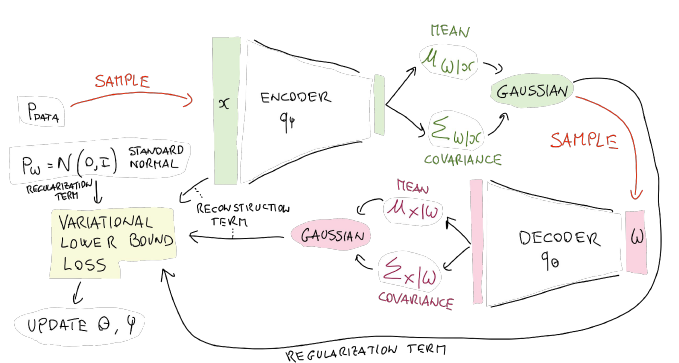
\includegraphics[width=0.8\linewidth]{imgs/chapter12/img14}
	\caption{Training in pratica}
	\label{fig:chapter12-14}
\end{figure}
\subsubsection{VAE condizionale}
Si assuma di avere un informazione $y\in\mathcal{Y}$ e si vuole generare nuovi dati sull'informazione.
Denota una distribuzione si probabilit\`a di encoding.
Si modifica il encoder e il decoder per prendere le informazioni in input ottenendo
$$q_\phi(\omega|x,y)$$
$$q_\theta(\omega|x,y)$$
Si definisce i priori condizionati sull'informazione $p_\omega(\omega|y)$.
Le VAE condizionali sono usate per direzionare l'output che si vuole dal generative model, altrimenti l'output seguirebbe solo la distribuzione di probabilit\`a dei dati. Esempio: dato un viso, generare il viso con occhiali.

\subsubsection{Probabilit\`a dei VAE}
\begin{itemize}
	\item Underfitting: agli stage iniziali il regolarizzatore \`e troppo forte e tende ad annullare la capacit\`a del modello.
	\item Blurry samples: il generatore tende a produrre data blurry in quanto la gaussiana tende a produrre blurry risultati.
\end{itemize}

\subsection{Generative adversarial Networks (GAN)}
Le GAN permettono di stimare la densit\`a implicitamente.
Si assuma di avere una densit\`a a priori $p_\omega\in\Delta(\Omega)$ e un generatore o decoder $g_\theta\in X^\Omega$ che genera i data points in $X$ dato un random point da $\Omega$ \ref{fig:chapter12-15}.
\begin{figure}
	\centering
	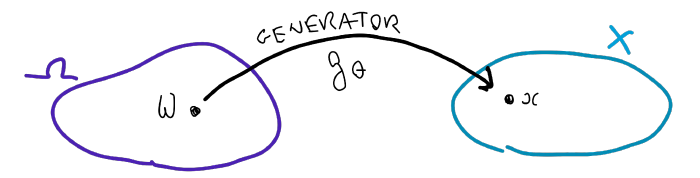
\includegraphics[width=0.6\linewidth]{imgs/chapter12/img15}
	\caption{Generative Adversarial Networks (GAN)}
	\label{fig:chapter12-15}
\end{figure}
Il generatore campiona direttametne dalla distribuzione implicita che non si conosce.
La densit\`a \`e indotta da $p_\omega$ e il generatore $g_\theta$ \`e dato da $q_\theta(x) = \mathbb{E}_{\omega\sim p_\omega}\delta[g_\theta(\omega) - x]$ dove $\delta$ \`e la funzione delta di Dirac.
L'obiettivo di GAN \`e trovare $\theta^*$ tale che $q_{\theta^*}$ che fitta meglio la distribuzione $p_{data}$ sotto la divergenza di Jensen-Shannon $d_{jS}$:
$$\theta^*\in arg\min\limits_{\theta} d_{JS}(p_{data},q_\theta)$$
Dove:
$$d_{JS}(p,q) = \frac{1}{2}d_{KL}\bigl(p,\frac{p+q}{2}\bigr)+\frac{1}{2}d_{KL}\bigl(q,\frac{p+q}{2}\bigr)$$
Che \`e chiaramente intrattabile da computare in quanto richiama la convergenza $KL$.
Lo stesso vale per il gradiente.

\subsubsection{Forma equivalente della divergenza JS}
\begin{align*}
	d_{JS}(p,q) &= \frac{1}{2}d_{KL}\bigl(p, \frac{p+q}{2}\bigr) + \frac{1}{2}d_{KL}\bigl(q, \frac{p+q}{2}\bigr)=\\
	&=\frac{1}{2}\mathbb{E}_{x\sim p}\bigl[\log\frac{2p(x)}{p(x)+q(x)}]\bigr]+\frac{1}{2}\mathbb{E}_{x\sim q}\bigl[\log\frac{2q(x)}{p(x)+q(x)}\bigr]=\\
	&=\frac{1}{2}\mathbb{E}_{x\sim p}\bigl[\log\frac{p(x)}{p(x)+q(x)}]\bigr]+\frac{1}{2}\mathbb{E}_{x\sim q}\bigl[\log\frac{q(x)}{p(x)+q(x)}\bigr] + \log(2)=\\
	&=\log(2)+\frac{1}{2}\max\limits_t\{\mathbb{E}_{x\sim p}[\log t(x)]+\mathbb{E}_{x\sim q}[\log(1-t(x))]\}
\end{align*}
Si deve pertanto imparare $t(x)$, un binary classifier che predice se $x$ deriva da $p$ o $q$.

\subsubsection{Obiettivo della GAN}
Sia $t_\varphi$ un classificatore o discriminatore per i data points in $\mathcal{X}$.
Allora si trova il limite inferiore sull'obiettivo:
\begin{align*}
	d_{JS}(p_{data}, q_\theta) &= \log(2) + \frac{1}{2}\max\limits_t\{\mathbb{E}_{x\sim p_{data}}[\log t(x)] + \mathbb{E}_{x\sim q_\theta}[\log(1-t(x))]\}\ge\\
	&= \log(2) + \frac{1}{2}\max\limits_\varphi\{\mathbb{E}_{x\sim p_{data}}[\log t_\varphi(x)] + \mathbb{E}_{x\sim q_\theta}[\log(1-t_\varphi(x))]\}
\end{align*}
Si possono ignorare $\frac{1}{2}$ e $\log(2)$ in quanto non cambiano il minimo.
Si deve pertanto minimizzare per ottenere il parametro del generatore $\theta^*$:
$$\theta^*\in arg\min\limits_\theta\max\limits_\varphi\{\mathbb{E}_{x\sim p_{data}}[\log t_\phi(x)] + \mathbb{E}_{x\sim q_\theta}[\log(1-t_\theta(x))]\}$$
Anche in questa forma \`e intrattabile in quanto dipende dalla densit\`a specifica di $q_\theta$, ma:
\begin{align*}
	\mathbb{E}_{x\sim q_\theta}[f(x)] &= \int q_\theta(x)f(x)dx = \iint\delta[g_\theta(\omega)-x]p_\omega(\omega)d\omega f(x)dx=\\
	& = \iint\delta[g_\theta(\omega)-x]f(x)dxp_\omega d\omega = \int f(g_\theta(\omega))p_\omega(\omega)d\omega = \\
	&= \mathbb{E}_{\omega\sim p_\omega}[f(g_\theta(\omega))]
\end{align*}
Da cui si pu\`o sostituire con $g_\theta$:
$$\theta^*\in arg\min\limits_{\theta}\{\mathbb{E}_{x\sim p_{data}}[\log t_\phi(x)]+\mathbb{E}_{\omega\sim p_\omega}[\log(1-t_\phi(g_\theta(\omega)))]\}$$

\subsubsection{Game theoretic interpretation}
Questo pu\`o essere visto come un gioco a due giocatori in cui il giocatore 1 o il generatore tenta di generare i dati che non possono essere distinte dai dati veri.
Il giocatore 2 \`e il discriminatore che cerca di indovinare se l'input viene dalla vera distribuzione o \`e falso.
Il payoff \`e preso con segno positivo per il discriminatore e negativo per il generatore.
Pertanto \`e descritto come un gioco non cooperativo a due giocatori e zero somma.
Il payoff \`e pertanto:
$$V(\theta,\varphi) = \mathbb{E}_{x\sim p_{data}}[\log t_\varphi(x)]+\mathbb{E}_{x\sim p_\omega}[\log(1-t_\varphi(g_\theta(\omega)))]$$
Si pu\`o pertanto scrivere il problema di minmax come:
$$\theta^*\in V(\theta,\varphi)$$

\begin{figure}
	\centering
	\begin{minipage}{.5\textwidth}
		\centering
		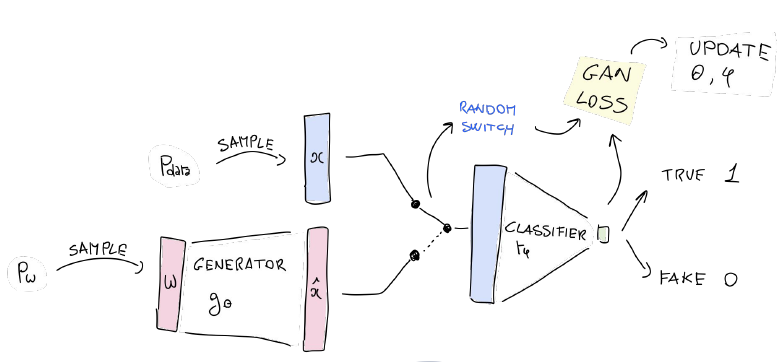
\includegraphics[width=1\linewidth]{imgs/chapter12/img16}
		\caption{Training}
		\label{fig:chapter12-16}
	\end{minipage}%
	\begin{minipage}{.5\textwidth}
		\centering
		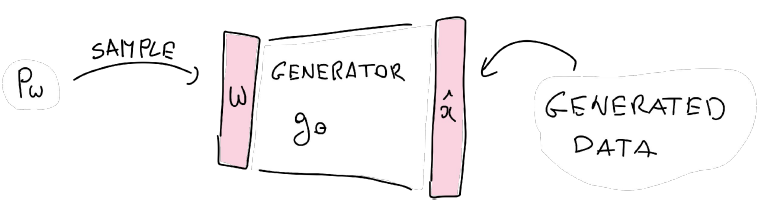
\includegraphics[width=1\linewidth]{imgs/chapter12/img17}
		\caption{Testing}
		\label{fig:chapter12-17}
	\end{minipage}
\end{figure}

\subsubsection{Ottimizzazione}
Il gradiente del obiettivo del GAN rispetto ai parametri del generatore $\theta$ $\frac{\partial}{\partial\theta}\max_\varphi V(\theta,\varphi)$ e richiede la risoluzione del problema di massimizzazione con rispetto al parametro del discriminatore $\varphi$.
Questo dovrebbe essere proibitivo computazionalmente.
In pratica si alterna uno step di update per il generatore dopo $k$ update per il discriminatore, senza garanzia di convergenza.

\paragraph{Esempio con vanilla SGD}
\begin{multicols}{2}
	\begin{itemize}
		\item Il discriminatore si aggiorna $k$ volte: $\varphi = \varphi + \nu\frac{\partial}{\partial\varphi}V(\theta,\varphi)$.
		\item Il generatore si aggiorna $\theta = \theta-\nu\frac{\partial}{\partial\theta}V(\theta,\varphi)$
	\end{itemize}
\end{multicols}
Le aspettative nei gradienti con rispetto a $p_{data}$ e a $p_\omega$ sono stimate su mini-batch.

\subsubsection{Problemi con GAN}
\begin{itemize}
	\item Training stability: i parametri oscillano e non convergono.
	\item Mode collapse: il generatore potrebbe imparare a perfezionare pochi esempi dal training set e riprodurre solo quegli esempi per vincere sempre.
	\item Vanishing gradient: se il discriminatore \`e molto bravo e lascia il generatore con poco gradiente per imparare.
\end{itemize}

\subsubsection{Altri tipi di GAN}
Diversi modelli simili a GAN possono essere costruiti considerando diverse divergenze tra le probabilit\`a e applicando trucchi simili per eliminare la necessit\`a di conoscere la densit\`a esplicitamente:
\begin{multicols}{2}
	\begin{itemize}
		\item \emph{f-GANS} costruite su f-divergenza.
		\item \emph{b-GANS} costruite su Bergman divergenza.
		\item \emph{Wasserstein GAN} utilizzano la Wasserstein metric.
		\item Altre GAN possono essere derivate utilizzando altre metriche integrali di probabilit\`a.
		\item \emph{f-GANS} su f-divergenza.
	\end{itemize}
\end{multicols}
GAN e VAE possono essere combinate e GAN condizionali esistono che lavorano simile a VAE continual.
